The second model is an improved version using roughly the same architecture as the first, but adding dropout to reduce overfitting, batch normalization and another dense fully connected layer.
\begin{center}
    \begin{verbatim}
    Model: "sequential_3"
    _________________________________________________________________
    Layer (type)                 Output Shape              Param #   
    =================================================================
    conv2d_18 (Conv2D)           (None, 32, 32, 32)        896       
    _________________________________________________________________
    batch_normalization_12 (Batc (None, 32, 32, 32)        128       
    _________________________________________________________________
    conv2d_19 (Conv2D)           (None, 32, 32, 32)        9248      
    _________________________________________________________________
    batch_normalization_13 (Batc (None, 32, 32, 32)        128       
    _________________________________________________________________
    max_pooling2d_9 (MaxPooling2 (None, 16, 16, 32)        0         
    _________________________________________________________________
    dropout_8 (Dropout)          (None, 16, 16, 32)        0         
    _________________________________________________________________
    conv2d_20 (Conv2D)           (None, 16, 16, 64)        18496     
    _________________________________________________________________
    batch_normalization_14 (Batc (None, 16, 16, 64)        256       
    _________________________________________________________________
    conv2d_21 (Conv2D)           (None, 16, 16, 64)        36928     
    _________________________________________________________________
    batch_normalization_15 (Batc (None, 16, 16, 64)        256       
    _________________________________________________________________
    max_pooling2d_10 (MaxPooling (None, 8, 8, 64)          0         
    _________________________________________________________________
    dropout_9 (Dropout)          (None, 8, 8, 64)          0         
    _________________________________________________________________
    conv2d_22 (Conv2D)           (None, 8, 8, 128)         73856     
    _________________________________________________________________
    batch_normalization_16 (Batc (None, 8, 8, 128)         512       
    _________________________________________________________________
    conv2d_23 (Conv2D)           (None, 8, 8, 128)         147584    
    _________________________________________________________________
    batch_normalization_17 (Batc (None, 8, 8, 128)         512       
    _________________________________________________________________
    max_pooling2d_11 (MaxPooling (None, 4, 4, 128)         0         
    _________________________________________________________________
    dropout_10 (Dropout)         (None, 4, 4, 128)         0         
    _________________________________________________________________
    flatten_3 (Flatten)          (None, 2048)              0         
    _________________________________________________________________
    dense_8 (Dense)              (None, 128)               262272    
    _________________________________________________________________
    dense_9 (Dense)              (None, 64)                8256      
    _________________________________________________________________
    dropout_11 (Dropout)         (None, 64)                0         
    _________________________________________________________________
    dense_10 (Dense)             (None, 10)                650       
    =================================================================
    Total params: 559,978
    Trainable params: 559,082
    Non-trainable params: 896
    _________________________________________________________________
    \end{verbatim}
\end{center}
This is a VGG-style network with 3 blocks compromised of 2 convolution layers and a pooling layer, followed by a dense fully connected layer for classification.
The ReLU\footnote{\href{https://machinelearningmastery.com/rectified-linear-activation-function-for-deep-learning-neural-networks/}{https://machinelearningmastery.com/rectified-linear-activation-function-for-deep-learning-neural-networks/}} activation function is used at each layer, and the loss function of the network is Cross Entropy\footnote{\href{https://www.tensorflow.org/api\_docs/python/tf/keras/losses/CategoricalCrossentropy}{https://www.tensorflow.org/api\_docs/python/tf/keras/losses/CategoricalCrossentropy}}
Batch Normalization is applied after each convolution layer.
Increasing dropout starting at 20\% after the first convolution block going up to 50\% at the final dense layer is applied.
This model resulted in an improved 85\% accuracy after 50 epochs, and as indicated by the learning curve, it can definitely benefit from more training epochs, and the overfitting problem from the previous model is now gone.
\begin{center}
    \captionsetup{type=figure}
    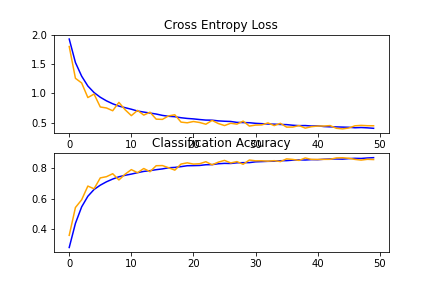
\includegraphics[width=250px]{sections/exp-2/images/improved-plot.png}
    \captionof{figure}{Model 1 - Cross Entropy Loss \& Classification Accuracy}
\end{center}
